\section{Experiments}
In this section, we construct the experimental evaluation and present the result analysis.

%\begin{table}[!htbp]
%\centering
%\caption{Datasets} \label{tab-data}
%\begin{tabular}{c|c|c}%
%\hline
%{Dataset} & {Time Interval} & {\#user} \\
%\hline
%\multirow{2}{*}{Ten Days} & {20180321 $\sim$ 20180331} & {1884174}\\
%\cline{2-3}
%\multirow{2}{*}{} & {20180501} & {177489}\\
%\hline
%\multirow{2}{*}{One Month} & {20180301 $\sim$ 20180331} & {5160229}\\
%\cline{2-3}
%\multirow{2}{*}{} & {20180501} & {177489}\\
%\hline
%\end{tabular}
%\end{table}

\subsection{Evaluation Dataset}
With the real-world datasets in Ant Credit Pay, an online credit payment service provided by Ant Financial Services Group,  we extract two sub-datasets for the evaluation, namely Ten Days Dataset (contains 1.88 million users ranging  from 2018/03/21 to 2018/03/31 for training) and One Month Dataset (contains 5.16 million users ranging from 2018/03/01 to 2018/03/31 for training). For both datasets, we predict the cash-out probability of users in 2018/05/01 (around 0.17 million users). In our datasets, we define the positive samples as users who have involved in suspected cash-out transactions within one month and the negative samples as users who have never involved in suspected cash-out transactions within one month. Since we utilize data in the next month when defining the label, the time interval between training and test set is one month. To be noted that since the cash-out fraud is very much in the minority among all transactions, the negative examples are sampled to keep the cash-out rate at around 2\% in our datasets.  

We construct an attributed heterogeneous information network based on the two datasets, consisting of  56.75 million users and 0.51 million merchants. In addition, the AHIN contains 77.40 million fund transfer relations between users and 20.64 million transaction relations between users and merchants. 
%consisting of multiple type of entities (\ie user (around 56.75 million) and merchant (around 507.51 thousand)) and relations (\ie fund transfer (around 77.40 million) and transaction (around 20.64 milion)) 
We extract 123 attributes for each user, including user profile, credit history, transaction summarizing, recent behaviors in other relative businesses and so on. Considering the scale of attribute value and the existence of missing value, we preproccess the two datasets with feature discretization.  

\begin{table}[t]
\footnotesize
\centering
\caption{Selected meta-paths and meta-path based neighbors statistics. } \label{tab-mp}
\begin{tabular}{c|c}%
\hline
\multirow{2}{*}{Meta-paths} & {\#Neighbors }\\%
\multirow{2}{*}{} & {(Min / Max / Avg.)} \\
\hline
{User-\scriptsize (transaction) -\small Merchant-\scriptsize (transaction)\small -User} & {1 / 16860 / 309}\\
\hline
{User-\scriptsize (fund transfer) \small-User}& {1 / 26235 / 150}\\
\hline
{User-\scriptsize (transaction) \small-Merchant} & {1 / 81 / 4} \\
\hline
\end{tabular}
\end{table}

\subsection{Evaluation Metrics}
We use the widely adopted metric to measure the performance of cash-out user detection , namely \textbf{AUC} (\ie Area Under the ROC Curve). The AUC metric is defined is:
\begin{equation}
AUC = \frac{\sum_{u \in \mathcal{U}^+}{rank_{u}} - \frac{|\mathcal{U}^+| \times (|\mathcal{U}^+| + 1)}{2}}{|\mathcal{U}^+| \times |\mathcal{U}^-| }.
\end{equation}
Here, $\mathcal{U}^+$ and $\mathcal{U}^-$ denotes the positive and negative set in the test set, respectively. And $rank_u$ indicates the rank of user $u$ via the score of prediction.


\begin{table*}[t]
\centering
\caption{Results of effectiveness experiments on two datasets \wrt the dimension of latent represantation $d$. A larger value indicates a better performance.} \label{tab-eff}
\begin{tabular}{c|c|c|c|c|c|c|c|c}%
\hline
\multirow{3}{*}{Algorithm} & \multicolumn{8}{|c}{AUC}\\
\cline{2-9}
\multirow{3}{*}{} & \multicolumn{4}{|c}{Ten Days Dataset} & \multicolumn{4}{|c}{One Month Dataset}\\
\cline{2-9}
\multirow{3}{*}{} & {$d = 16$} & {$d = 32$} & {$d = 64$} & {$d = 128$} & {$d = 16$} & {$d = 32$} & {$d = 64$} & {$d = 128$}\\
\hline
Node2vec & 0.5893  &0.5913 & 0.5926 & 0.5930 & 0.5980 & 0.6063 & 0.6009 & 0.6021\\
%\hline
Metapath2vec & 0.5914 & 0.5903 & 0.5917 & 0.5920 & 0.6005& 0.5976 &  0.5995 & 0.5983\\
%\hline
{Node2vec + Feature}  & 0.6455 & 0.6464  & 0.6510 & 0.6447 & 0.6541 & 0.6561 & 0.6607 & 0.6518\\
%\hline
{Metapath2vec + Feature}  & 0.6456 &  0.6429 & 0.6469 & 0.6485 & 0.6550 & 0.6552& 0.6523 & 0.6545\\
%\hline
Structure2vec & 0.6537 & 0.6556 & 0.6598 & 0.6545 & 0.6641 &0.6632 & 0.6657 & 0.6678\\
%\hline
GBDT & 0.6389 & 0.6389 & 0.6389 & 0.6389 & 0.6467 & 0.6467 & 0.6467 & 0.6467\\

GBDT$_{Struct}$& 0.6948 & 0.6948 & 0.6948 & 0.6948 & 0.6968 & 0.6968 & 0.6968 & 0.6968\\

HACUD & \textbf{0.7066} & \textbf{0.7115} & \textbf{0.7056}& \textbf{0.7049} &\textbf{0.7132} & \textbf{0.7160} & \textbf{0.7109}&\textbf{0.7154}\\
\hline
\end{tabular}
\end{table*}

\subsection{Methods to Compare}
We consider several representative methods for the cash-out user detection task,
%The selected baselines have a comprehensive coverage of existing methods for our scene, 
%We consider two kinds of representative recommendation methods
which  can roughly be categorized into three type: (1) Attribute only or Structure only (GBDT, Node2vec, Metapath2vec). (2) Structure + Attribute (Node2vec + Feature, Metapath2vec + Feature). (3) Structure + Attribute + Label (Structure2vec, GBDT$_{Struct}$).


\textbullet \textbf{Node2vec}~\citep{grover2016node2vec} : It is a representation learning method on homogeneous network. We employ it to learn representations for nodes, ignoring node heterogeneity, and feed them into a classification model.

\textbullet \textbf{Metapath2vec}~\citep{dong2017metapath2vec} : It is a heterogeneous information network embedding method for learning node embedding with meta-path guided random walks. Similarly, we also feed the node representations into a classification model.

\textbullet \textbf{Node2vec + Feature} : We feed the features of node as well as the embeddings learned by Node2vec into a classification model.

\textbullet \textbf{Metapath2vec + Feature} : We feed the features of node as well as the embeddings learned by Metapath2vec into a classification model.

\textbullet \textbf{Structure2vec}~\citep{dai2016discriminative} : It is an effective approach for network embedding based on network structure and feature information with labeled data.

\textbullet \textbf{GBDT}~\citep{friedman2001greedy} : It is a scalable tree-based model for feature learning and classification task. We feed node feature  into GBDT.

\textbullet \textbf{GBDT$_{Struct}$} : Besides node feature, we also feed the aggregate features of meta-path based neighbors into GBDT.

\subsection{Implementation Details}
We implement the proposed model based on Tensorflow~\citep{abadi2016tensorflow}.  We utilize two hidden layers for prediction. We randomly initialize the model parameters with a xavier initializer~\citep{glorot2010understanding} and choose RMSProp~\citep{tieleman2012lecture} as the optimizer. Moreover, we set the batch size to 256, the learning rate to 0.002 and set the regularizer parameter $\lambda = 0.01$ to prevent overfitting. We report the selected meta-paths and meta-path based neighbors statistics information in Table~\ref{tab-mp}. For the other comparison methods, we optimize their parameters according to literatures. Moreover, for all baselines, we implement them on parameter server based distributed learning systems\citep{zhou2017kunpeng} for scaling up to large-scale datasets. And we select GBDT as the final classification model for the baselines.


\subsection{Experimental Results}
\paratitle{Performance Comparison}. We report the comparison results of the proposed approach and baselines \wrt the dimension of latent representation $d$ in Table~\ref{tab-eff}. The major findings from the experimental results can be summarized as follows:

(1) Our model outperforms all the baselines, which indicates that our model adopts a more principled way to leverage interaction relations and attribute information for improving prediction performance. Our model achieves the best performance where the dimension of latent representation $d = 32$. And overall, the performance change trend is smooth, indicating that our model is not very sensitive to this parameter.

(2) Among these baselines, we can find that the overall performance order is as follows: (label + attribute + structure) based methods (\ie GBDT$_{Struct}$, Structure2vec) $>$ (attribute + structure) based methods (\ie Node2vec + Feature, Metapath2vec + Feature) $>$ structure or attribute only based method (\ie Node2vec, Metapath2vec, GBDT). 
It indicates that the better performances can be achieved through fusing more information. In addition, structure information (\ie interaction relations) is really helpful for performance improvement.
%which indicates the usefulness of attribute and label information.

(3) Compare the two variants of GBDT (\ie traditional GBDT and GBDT$_{Struct}$), we can find that GBDT$_{Struct}$ significantly outperforms traditional GBDT and other baselines, which further demonstrates the contribution of structural features provided by meta-path based neighbors in AHIN.




%Among these baselines, attribute based method (\ie Node2vec$_{feature}$, Metapath2vec$_{feature}$) is better than structure-only based method (\ie Node2vec, Metapath2vec), which indicates the usefulness of attributed information.

%\begin{figure}
%\begin{minipage}[t]{0.45\linewidth}
%\centering
%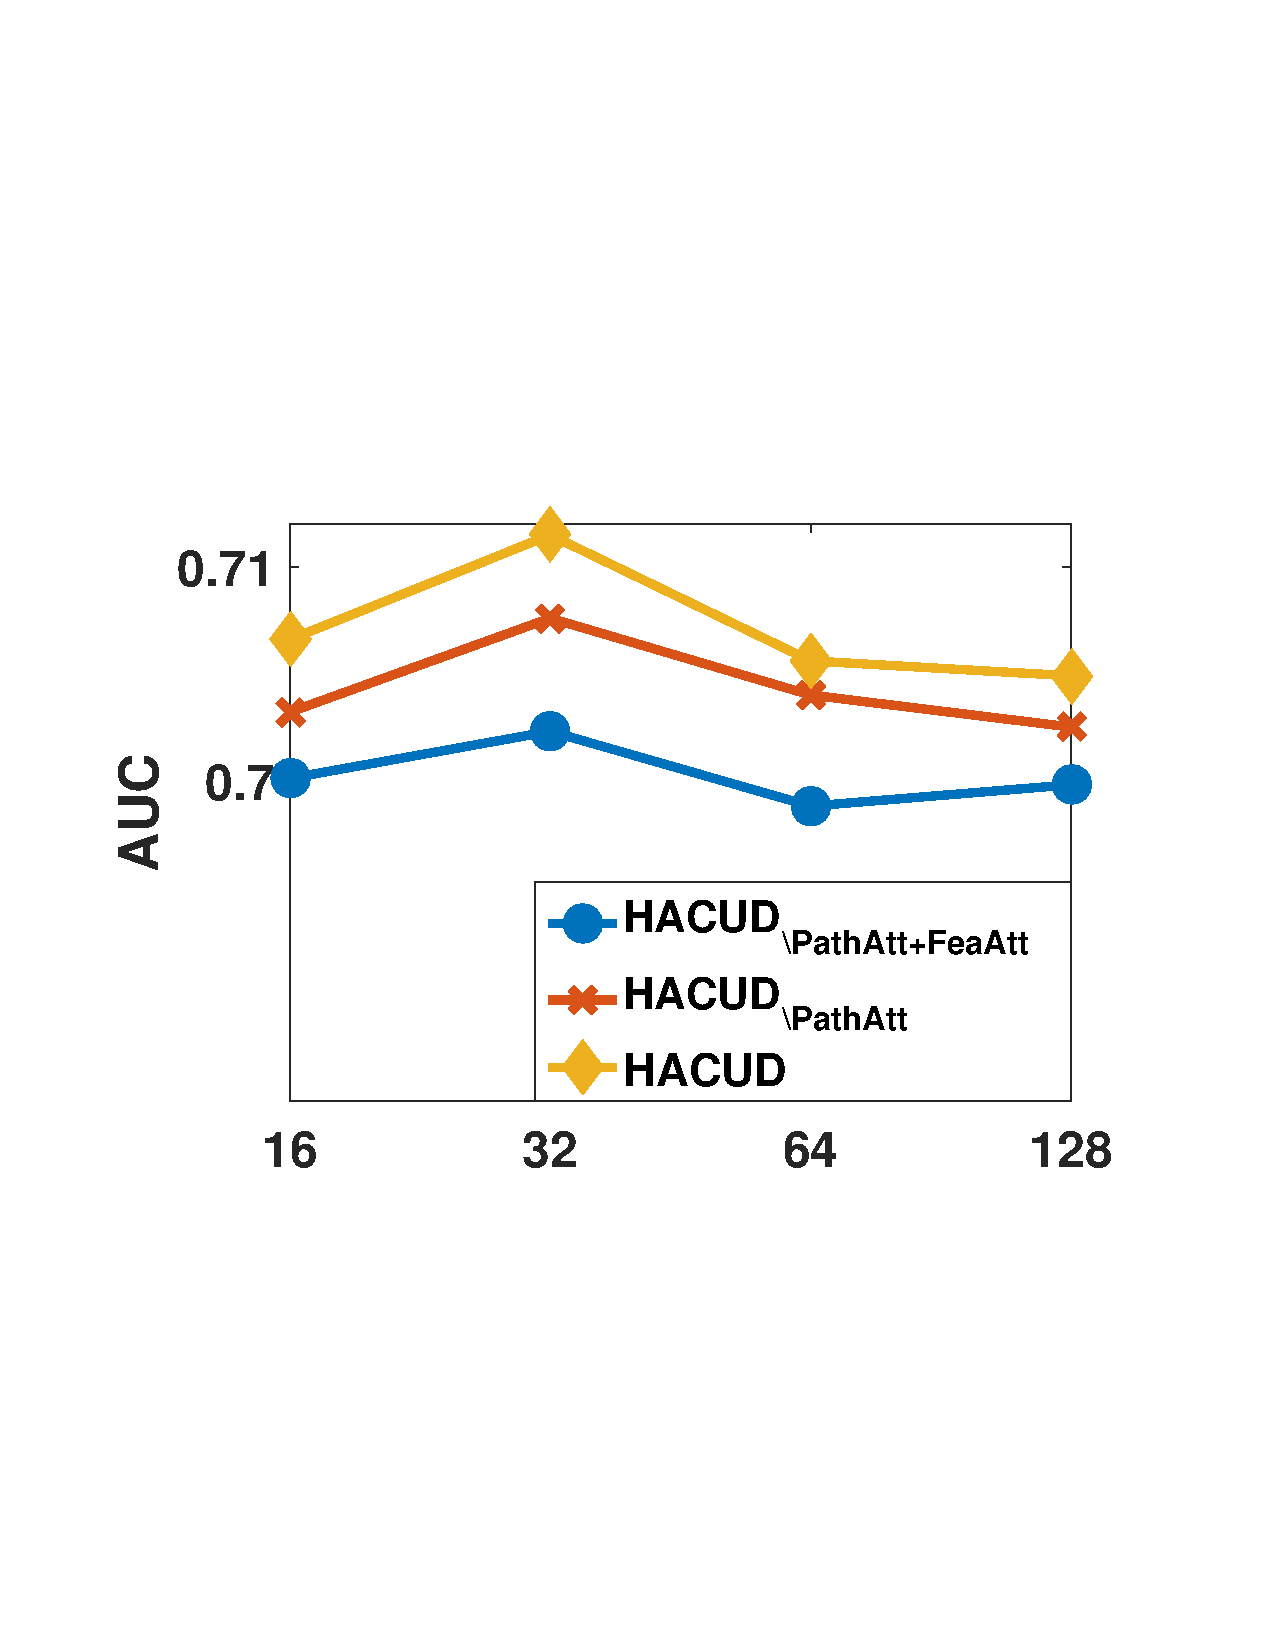
\includegraphics[width=4.0cm]{image/attention.pdf}
%\caption{Performance comparison of hierarchical attention \wrt the number of latent factors.}
%\label{fig-attention}
%\end{minipage}
%\begin{minipage}[t]{0.45\linewidth}
%\centering
%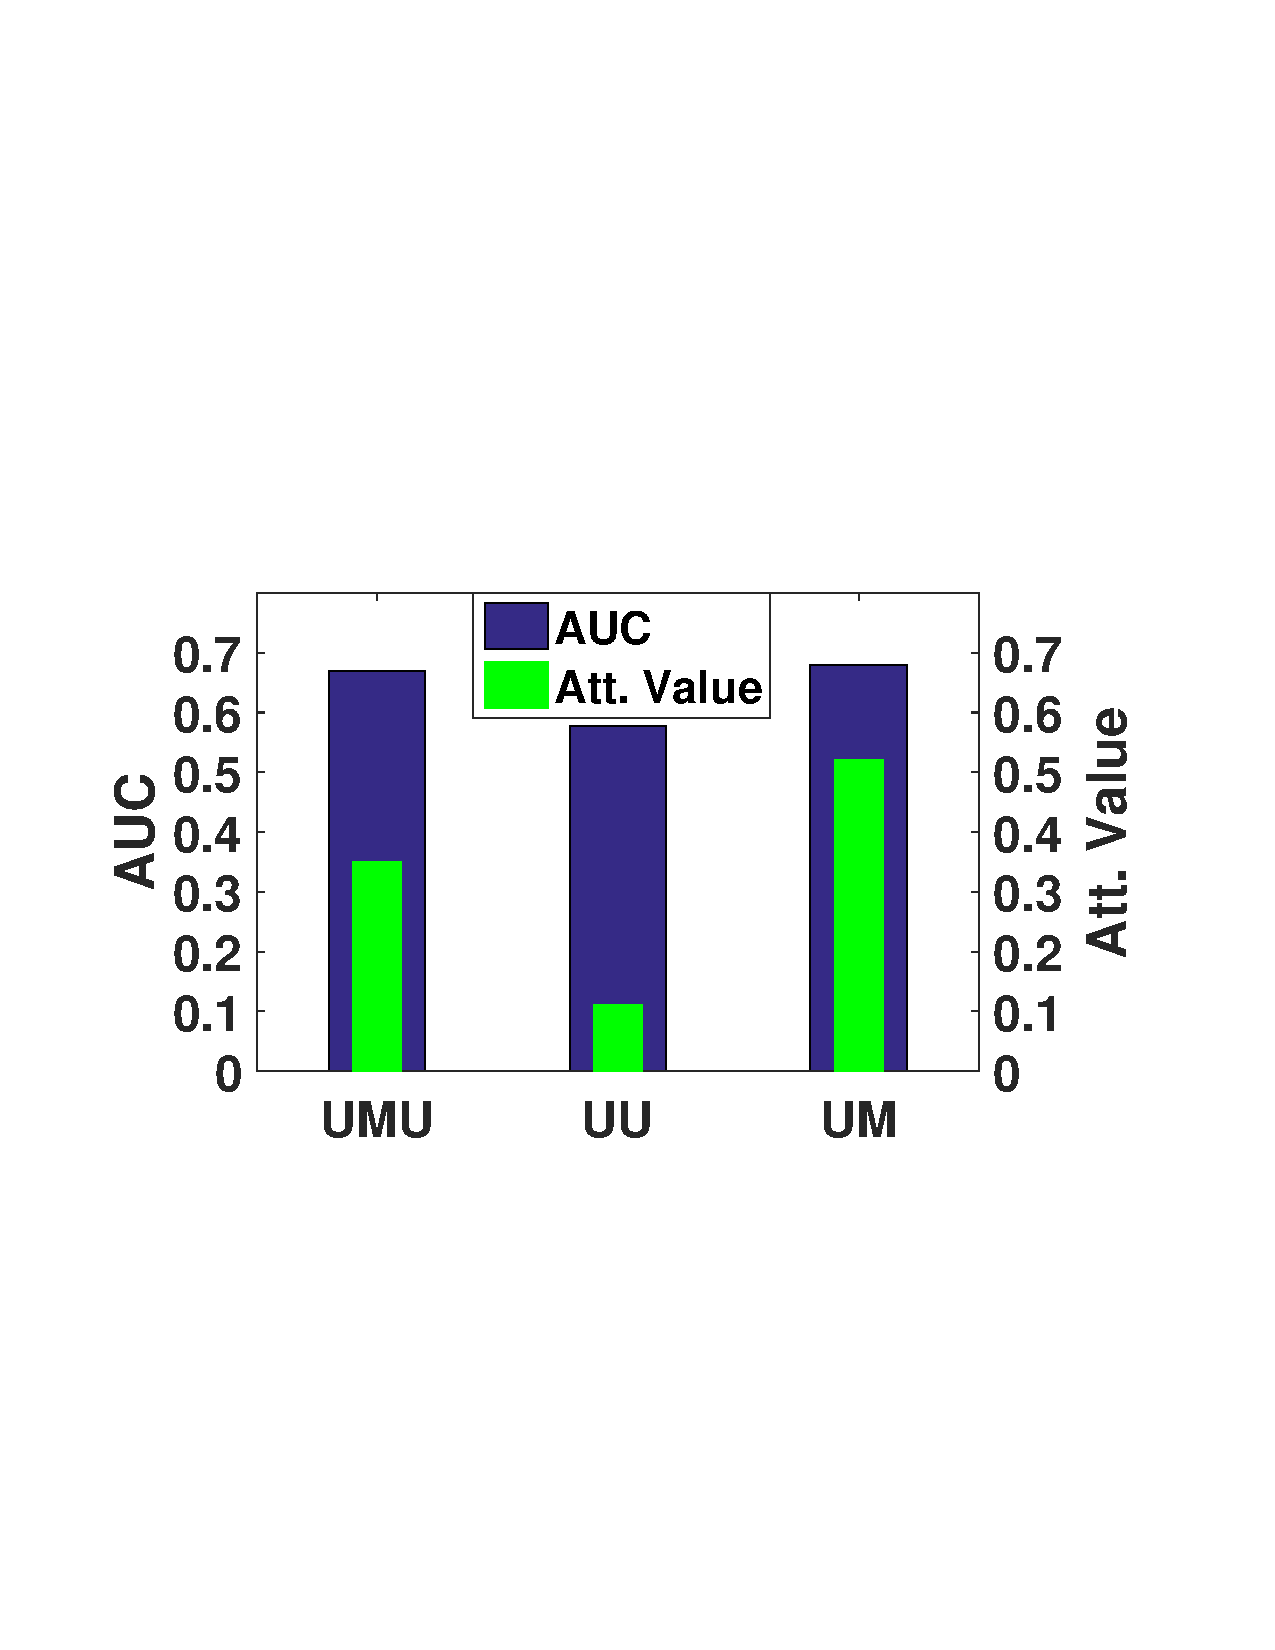
\includegraphics[width=4.6cm]{image/att_val.pdf}
%\caption{Comparison of performances on single meta-paths and the attention values of meta-paths.
%Meta-paths with better performances usually attract more attentions.
%}
%\label{fig-att_val}
%\end{minipage}
%\end{figure}

\begin{figure}[t]
\centering
\subfigure[Ten Days Dataset]{
\begin{minipage}[t]{0.45\linewidth}
\centering
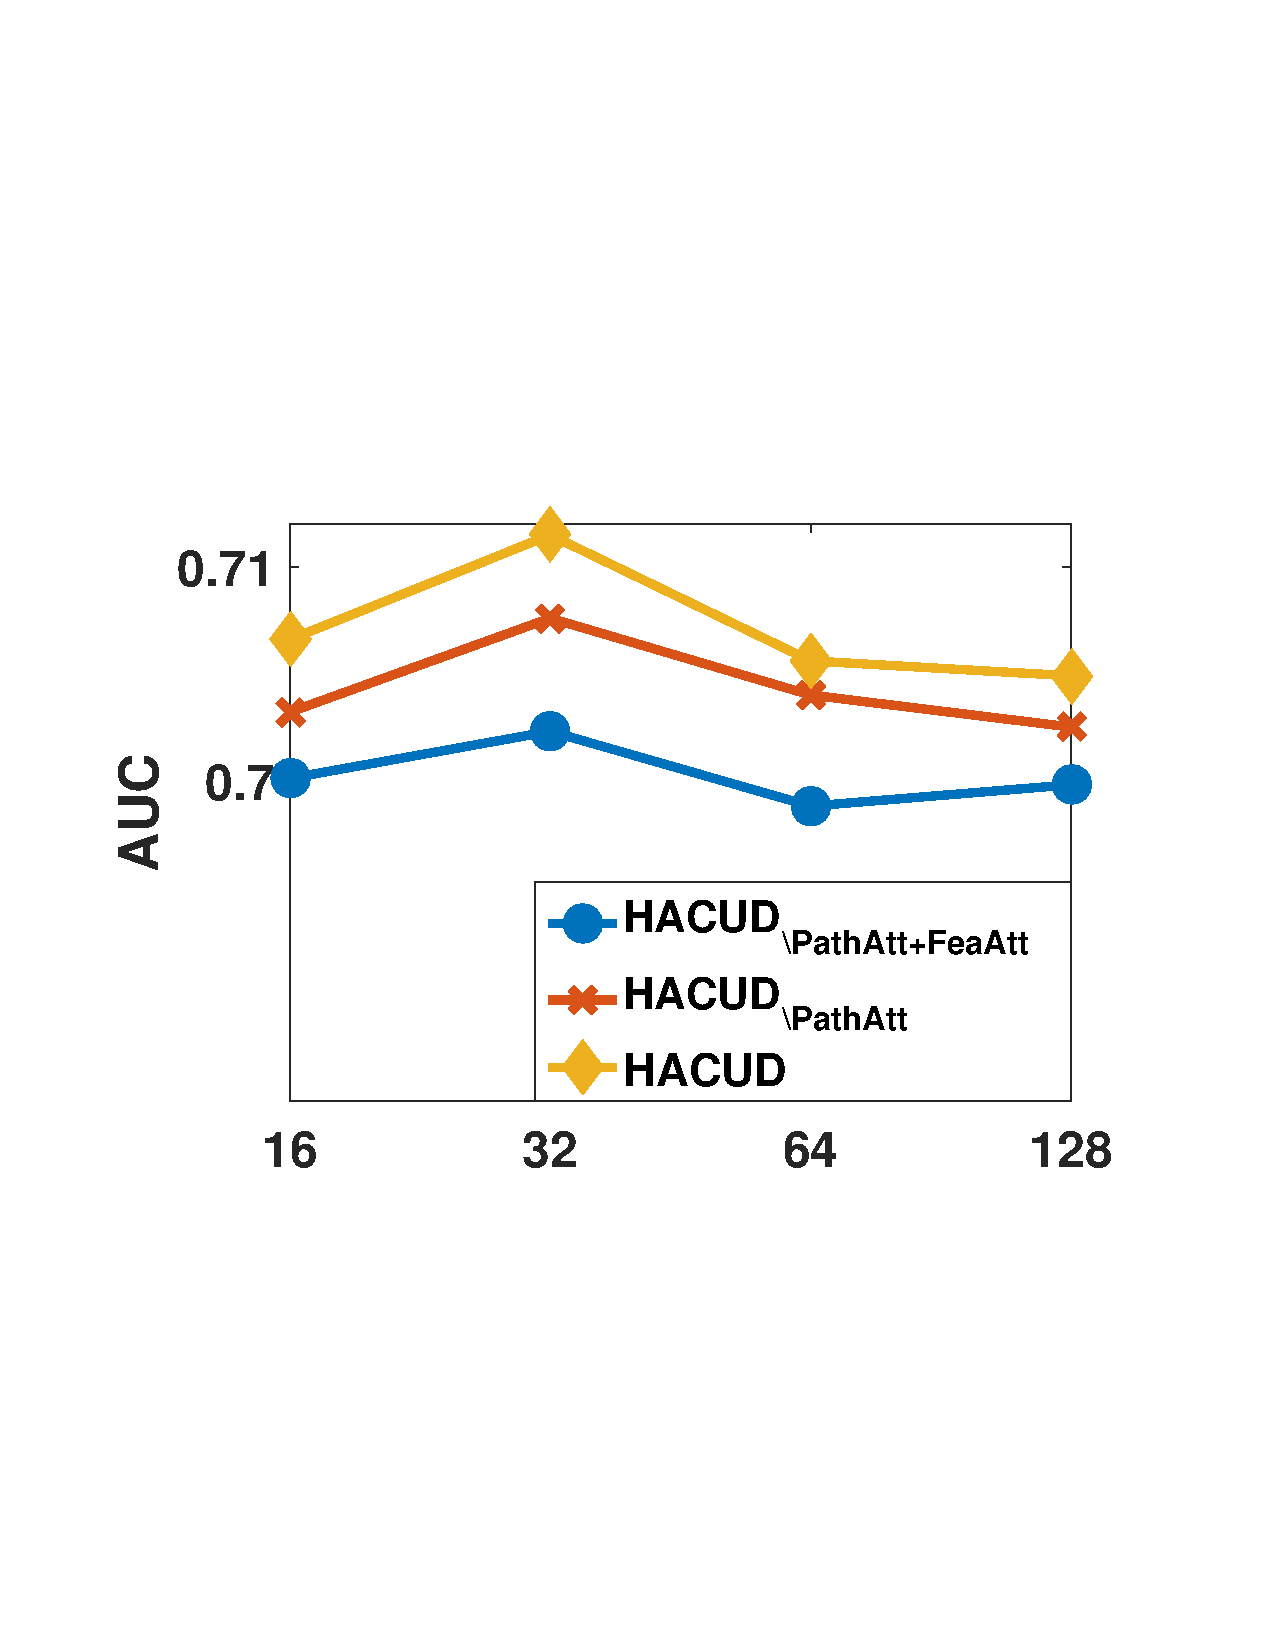
\includegraphics[width=4.1cm]{image/attention.pdf}
\end{minipage}
}
%\hspace{30pt}
\subfigure[One Month Dataset]{
\begin{minipage}[t]{0.45\linewidth}
\centering
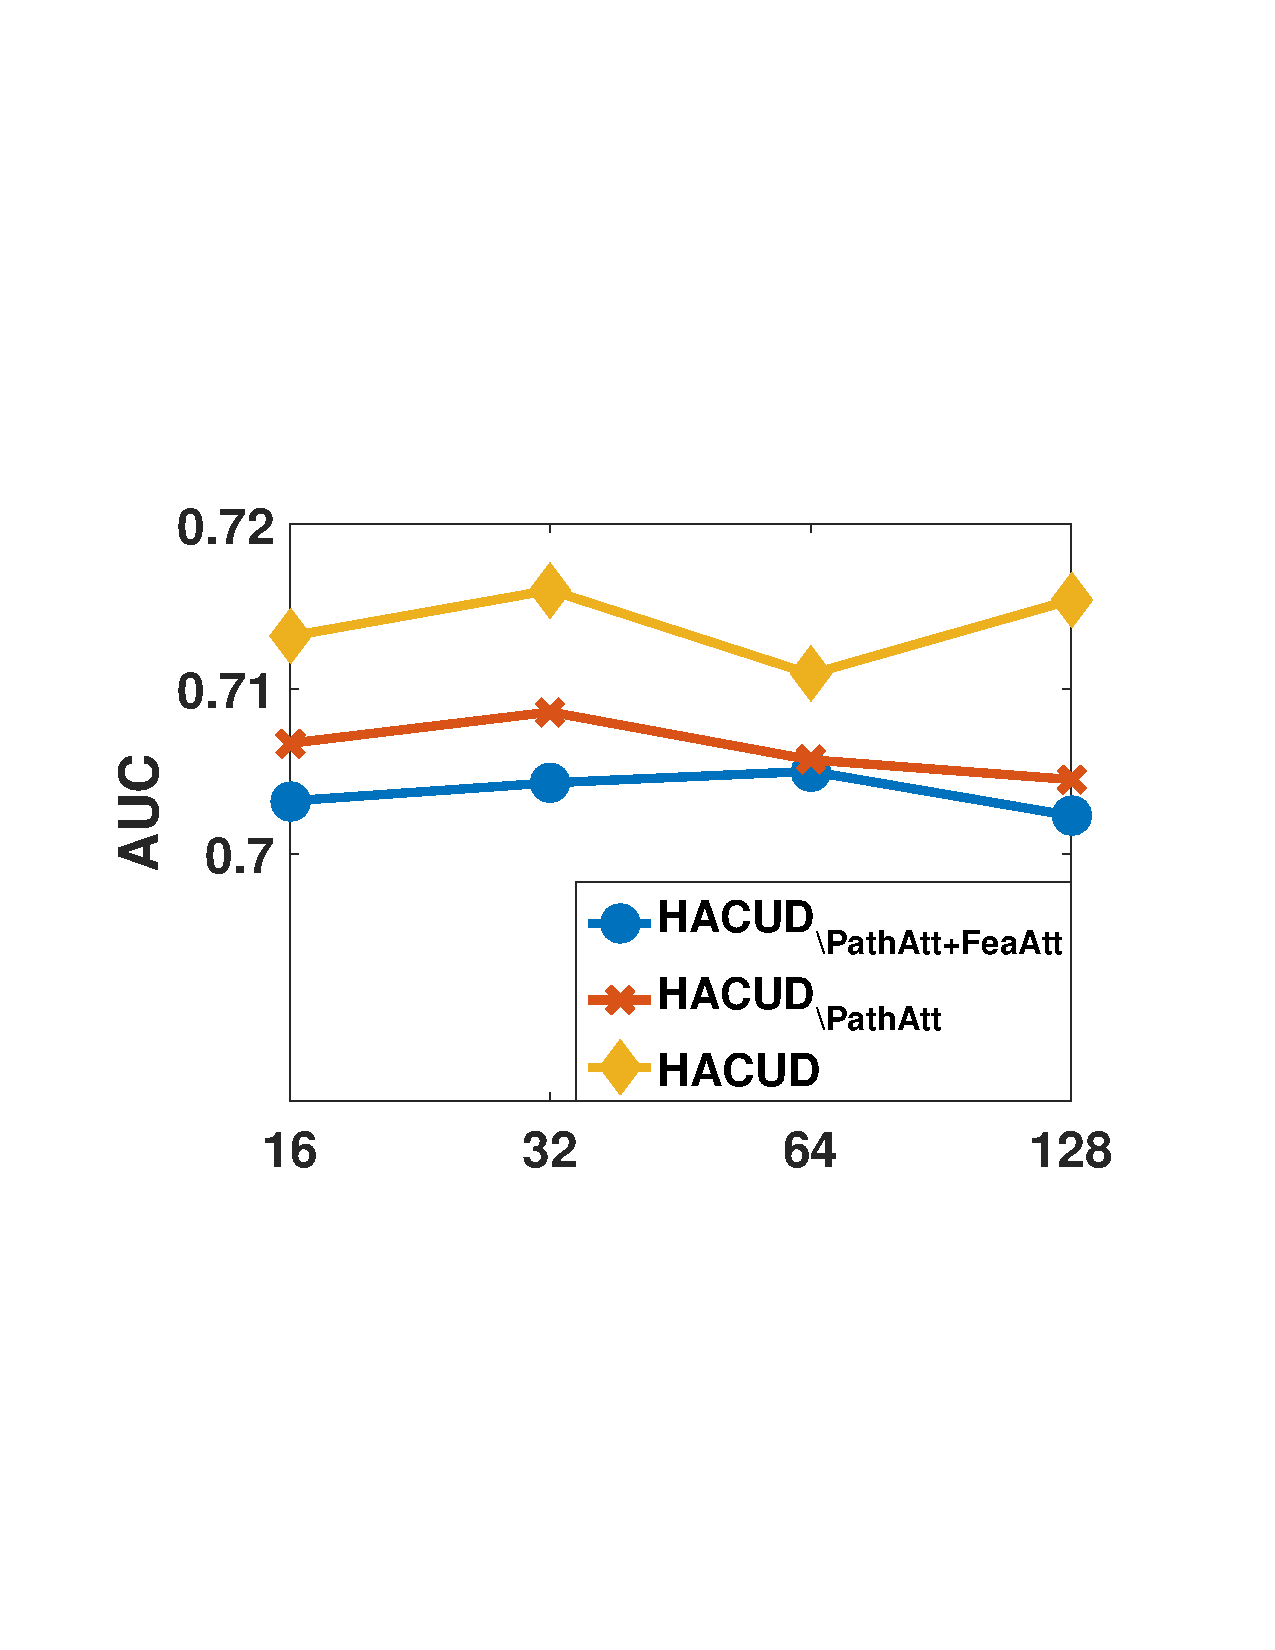
\includegraphics[width=4.1cm]{image/attention_large.pdf}
\end{minipage}
}
\caption{Performance comparison of hierarchical attention \wrt the dimension of latent representation $d$.\label{fig-attention}}
\end{figure}



\paratitle{Effects of Hierarchical Attention}. One of the major contributions of HACUD is hierarchical attention mechanism which learns the user preference towards features and meta-paths.
%is the incorporation of hierarchical attention mechanism, which takes the user's preference towards features and meta-paths into consideration for cash-out prediction. 
In order to examine its effectiveness, we compare our model with its two variants, namely HACUD$_{ \backslash PathAtt}$ (HACUD without path attention) and HACUD$_{\backslash PathAtt + FeaAtt}$ (HACUD without path and feature attention). 
For the performance comparison in Fig.~\ref{fig-attention}, 
%We report the performance comparison in the Fig.~\ref{fig-attention}. 
we can find that the overall performance order is as follows: HACUD $>$ HACUD$_{ \backslash PathAtt}$ $>$ HACUD$_{\backslash PathAtt + FeaAtt}$. The results show that the hierarchical mechanism is able to better utilize the user feature and features generated by meta-paths  in two aspects. First,  different meta-paths have different contributions to cash-out user prediction, which cannot be treated equally (\ie HACUD$_{ \backslash PathAtt}$). Second, each user tends to place different importance to the various attributes for each meta-path. Ignoring such influence may not be able to achieve the promising performance for fully exploiting attribute and structure information (\ie HACUD$_{\backslash PathAtt + FeaAtt}$).

Furthermore, we report the performances based on single meta path and corresponding average attention value in Fig.~\ref{fig-att_val}.  As we have observed, the performances of HACUD with different meta-paths and the corresponding attentions are positively correlated ( \ie important meta-paths tend to attract more attentions). In other words, the proposed HACUD model is potential to let different users focus on the proper meta-paths. %with the optimal performance, which reveal the effective of our path attention. %Obviously, the meta-path $UM$ and $UMU$ seem to be more important than others. One reasonable explanation is that cash-out users have aggregation effect.

\begin{figure}[t]
\centering
\subfigure[Ten Days Dataset]{
\begin{minipage}[t]{0.45\linewidth}
\centering
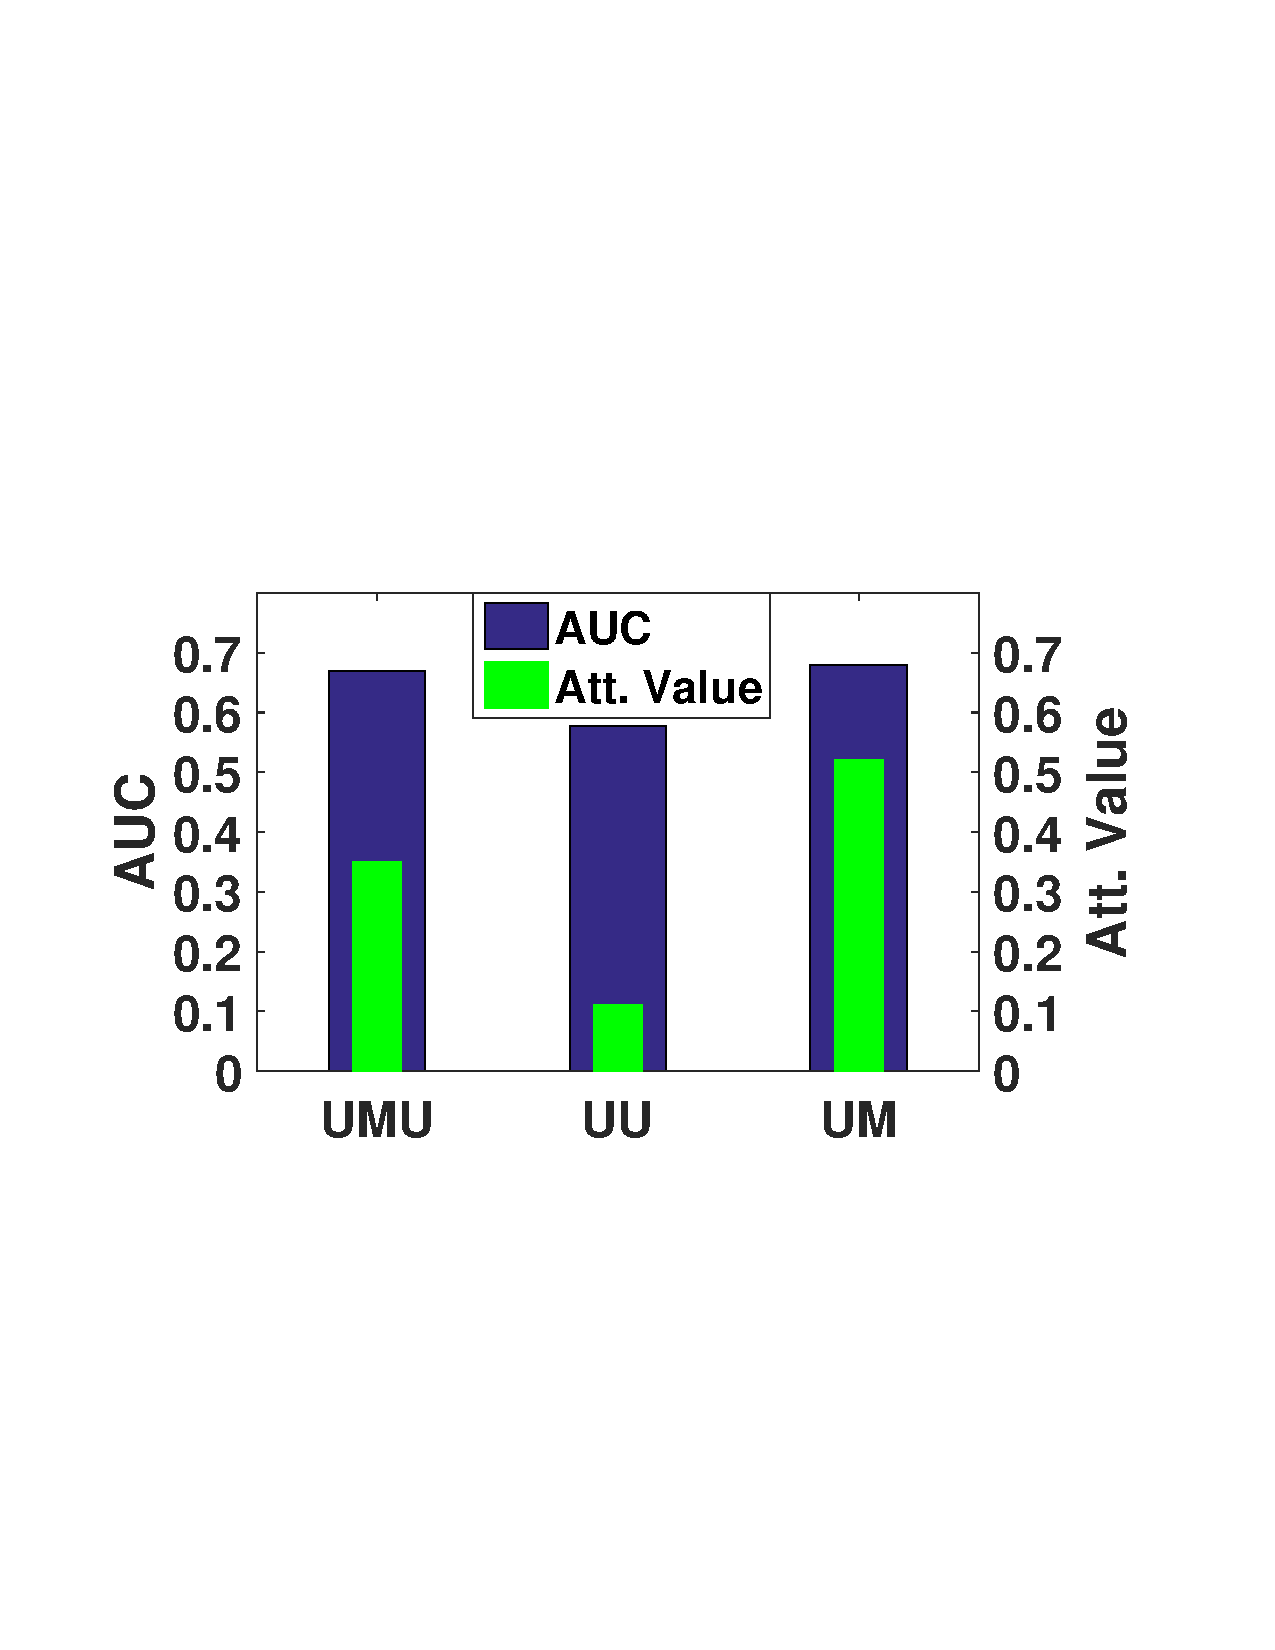
\includegraphics[width=4.2cm]{image/att_val.pdf}
\end{minipage}
}
%\hspace{30pt}
\subfigure[One Month Dataset]{
\begin{minipage}[t]{0.45\linewidth}
\centering
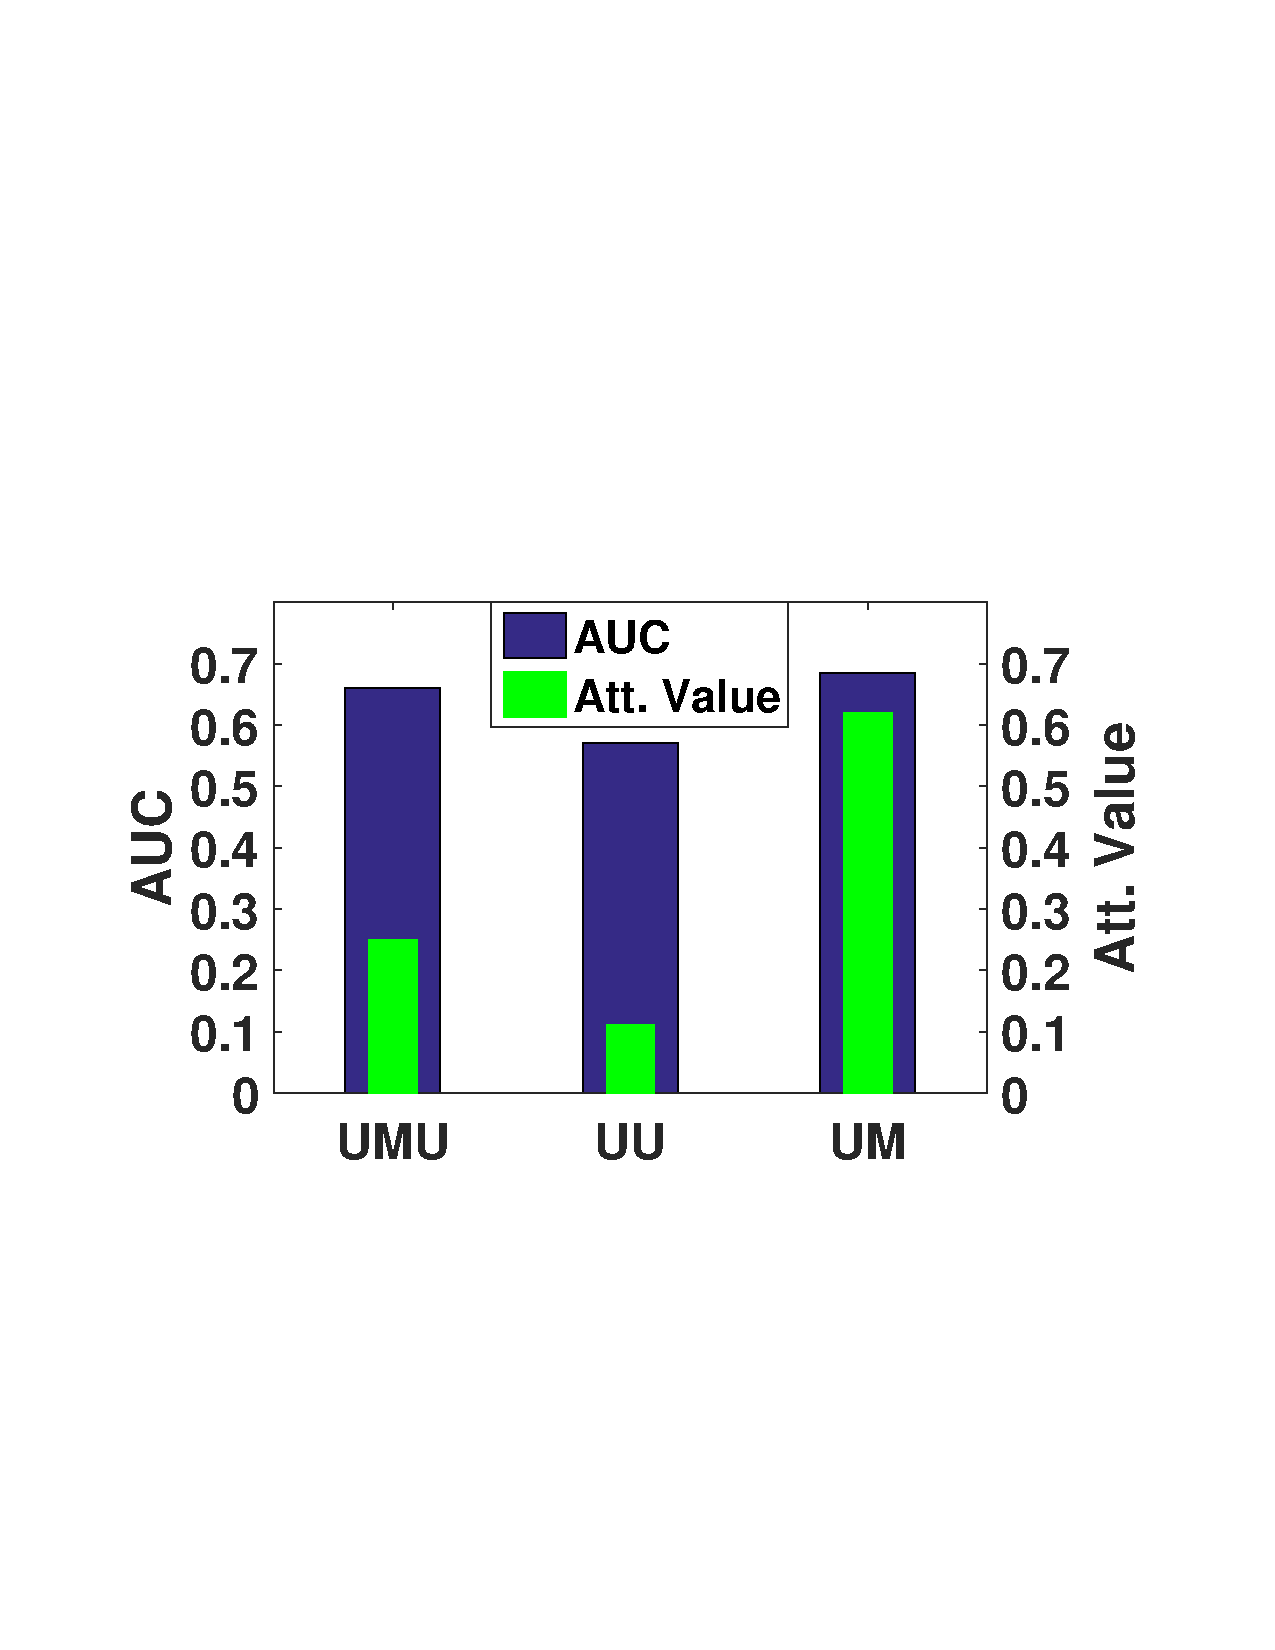
\includegraphics[width=4.0cm]{image/att_val_large.pdf}
\end{minipage}
}
\caption{Performances comparison on different meta-paths and corresponding attention values.\label{fig-att_val}}
\end{figure}
\paratitle{Impact of Different Meta-paths}.
As mentioned above, our model utilizes a selected set of meta-paths. To further analyze the impact of different meta-paths, we gradually incorporate  these meta-paths into our model and observe the performance change. In addition, we select GBDT as the baselines in this experiment. For convenience, we make the following denotation: (1) M$_1$ : user feature only; (2) M$_2$ : user feature + $UMU$; (3) M$_3$ : user feature + $UMU$ + $UU$; (3) M$_4$ : user feature + $UMU$ + $UU$ + $UM$.
As shown in the Fig.~\ref{fig-metapath}, we can observe that the performance would improve with the incorporation of more meta-paths, which demonstrates the effectiveness of structure information contained in different meta-paths. Specially, we can find that our model has a significant performance boost when adding the meta-paths $UMU$ and $UM$. This finding is consistent with previous observation in Fig.~\ref{fig-att_val}, where these two meta-paths have better performances, accompanying with higher attention values.


\paratitle{Parameter Tuning}
Besides the dimension of latent representation $d$ in Table~\ref{tab-eff}, our model also involves another important tuning parameter $\lambda$ in Eq.~\ref{equ-objective}.  We vary it in the set of  \{0.0, 0.0001, 0.001, 0.01, 0.1, 1.0\}. As shown in Fig. 5, the optimal performance is obtained near $\lambda = 0.01$, indicating that  $\lambda$ cannot be set too small or too large to prevent overfitting and underfitting.






